\section{Methodology}

\subsection{Multimodal Input Representation}
To avoid ambiguity between symbolic variables and sensor names, we represent each observation using an ordered multimodal feature vector:
\begin{equation}
\mathbf{x} = [x, y, \text{TEMP}, \text{COR}_{A}, \text{COR}_{V}] \in \mathbb{R}^{5},
\end{equation}
and a three-output target vector:
\begin{equation}
\mathbf{y} = [\text{pH}, \text{OD}, \text{TURB}] \in \mathbb{R}^{3}.
\end{equation}
Input features are normalized before spike encoding. We then apply rate coding so that each normalized scalar is converted into a spike train over $T$ time steps, with firing probability proportional to its magnitude. This produces a temporal representation compatible with the downstream LIF dynamics while preserving the multimodal structure of the original sample.

\subsection{SNN Architecture}
The model follows a feed-forward SNN with topology $5 \rightarrow 64 \rightarrow 3$, with a hidden leaky integrate-and-fire (LIF) layer, as illustrated in Fig.~\ref{fig:proposed_arch}. The membrane update is
\begin{equation}
\mathbf{u}_{t+1} = \beta\,\mathbf{u}_{t} + \mathbf{W}\mathbf{s}_{t} - \theta\,\mathbf{z}_{t},
\end{equation}
where $\beta$ is membrane decay, $\theta$ is firing threshold, and $\mathbf{z}_t$ are emitted spikes. Output prediction is computed by temporal aggregation across steps.

\begin{figure}[!htbp]
\centering
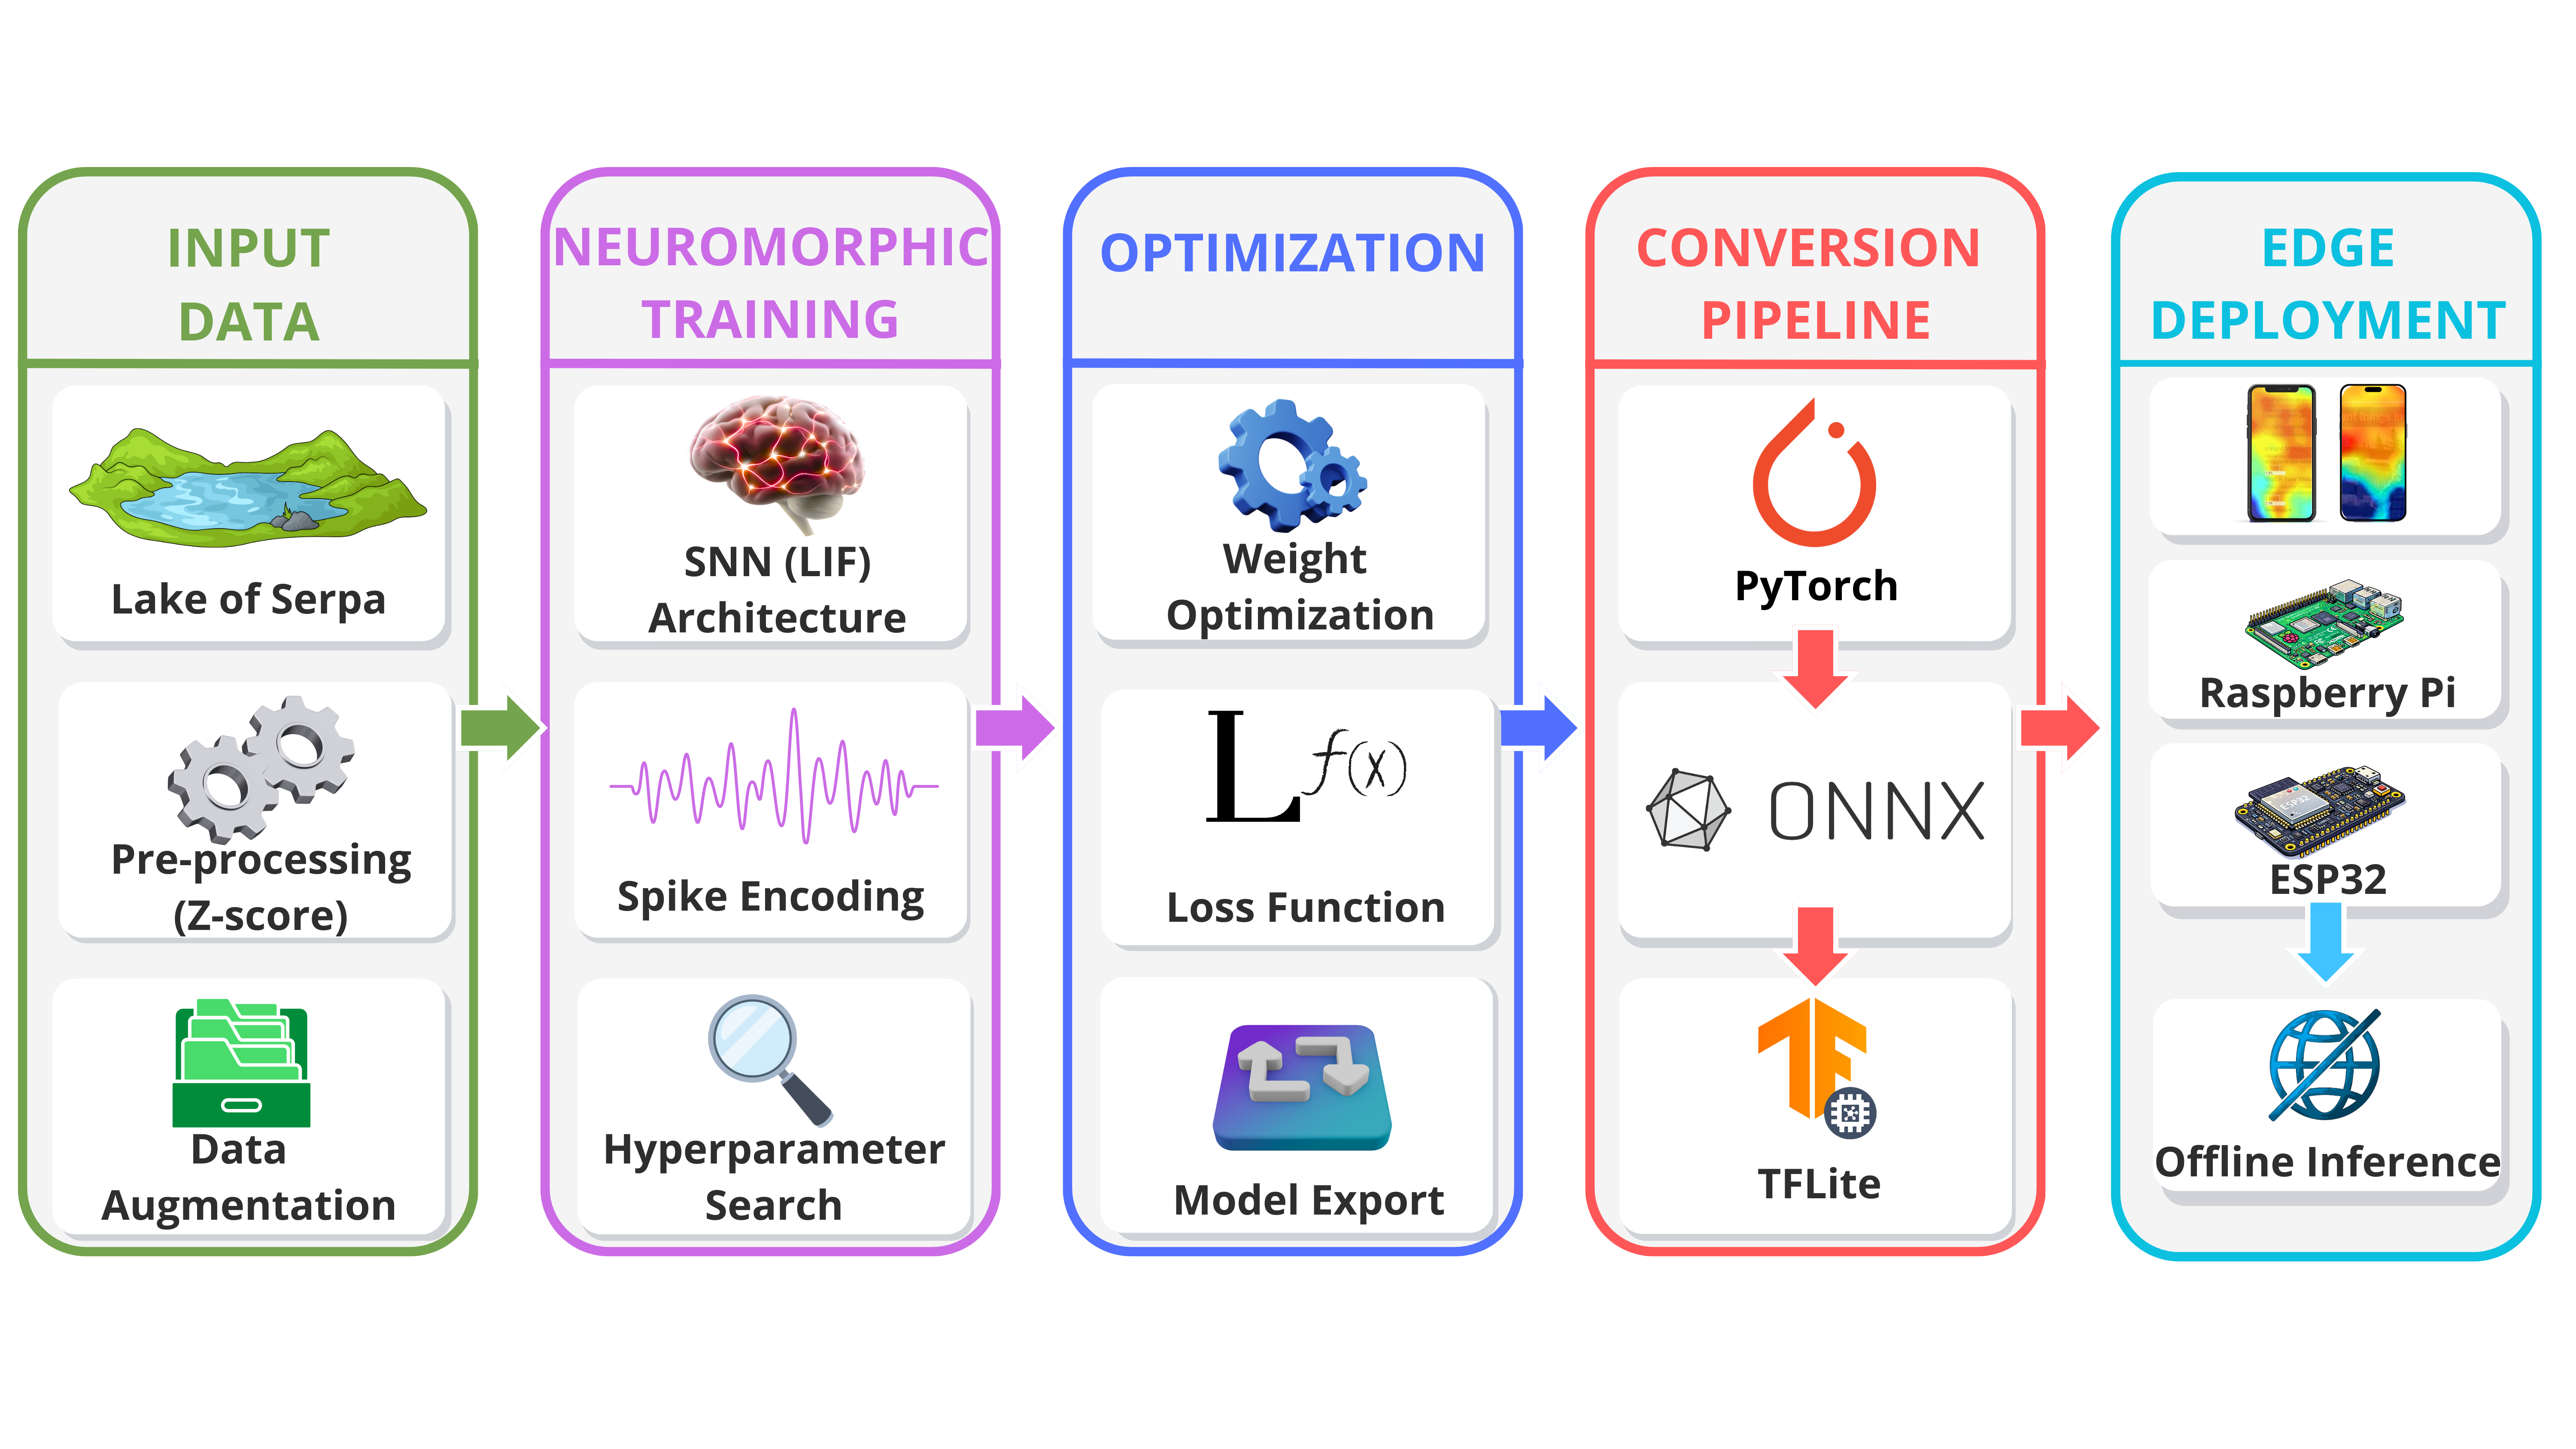
\includegraphics[width=\linewidth]{Arquitetura.png}
\caption{Proposed multimodal SNN architecture for offline edge inference.}
\label{fig:proposed_arch}
\end{figure}

Figure~\ref{fig:proposed_arch} presents the complete end-to-end workflow: field data preparation (normalization and controlled augmentation), neuromorphic training with LIF neurons and hyperparameter search, model optimization and export through the PyTorch$\rightarrow$ONNX$\rightarrow$TFLite interoperability path, and offline edge deployment on Android, Raspberry Pi, and ESP32.

\subsection{Training Protocol}
Training used Adam optimizer and weighted MSE loss with early stopping. Hyperparameters were selected by grid search over hidden size, learning rate, temporal steps $T$, threshold, and decay factor. \rev{The full search space was: hidden size $\in \{32, 64, 96\}$, $T \in \{10, 15, 25\}$, learning rate $\in \{0.0005, 0.001, 0.002\}$, decay $\beta \in \{0.90, 0.95\}$, threshold $\theta \in \{0.8, 1.0\}$, and augmentation noise $\sigma \in \{0.01, 0.02, 0.03\}$, totaling 324 configurations evaluated by validation loss. The selected configuration was hidden size 64, $T=15$, learning rate $0.002$, $\beta=0.95$, $\theta=0.8$, and $\sigma=0.01$.} Evaluation used repeated random seeds and macro metrics (MAE, RMSE, and $R^2$) over the three targets. \rev{The ten independent seeded runs implement repeated random subsampling validation, which approximates cross-validation behavior in this small-data regime; a full k-fold protocol is planned for the extended dataset in future campaigns.}

As shown in Fig.~\ref{fig:loss_curve_method}, training and validation losses decrease rapidly in the initial epochs and converge to a stable plateau with limited divergence, indicating consistent optimization without strong overfitting and supporting the use of early stopping in this small-data regime.

\begin{figure}[h!]
\centering
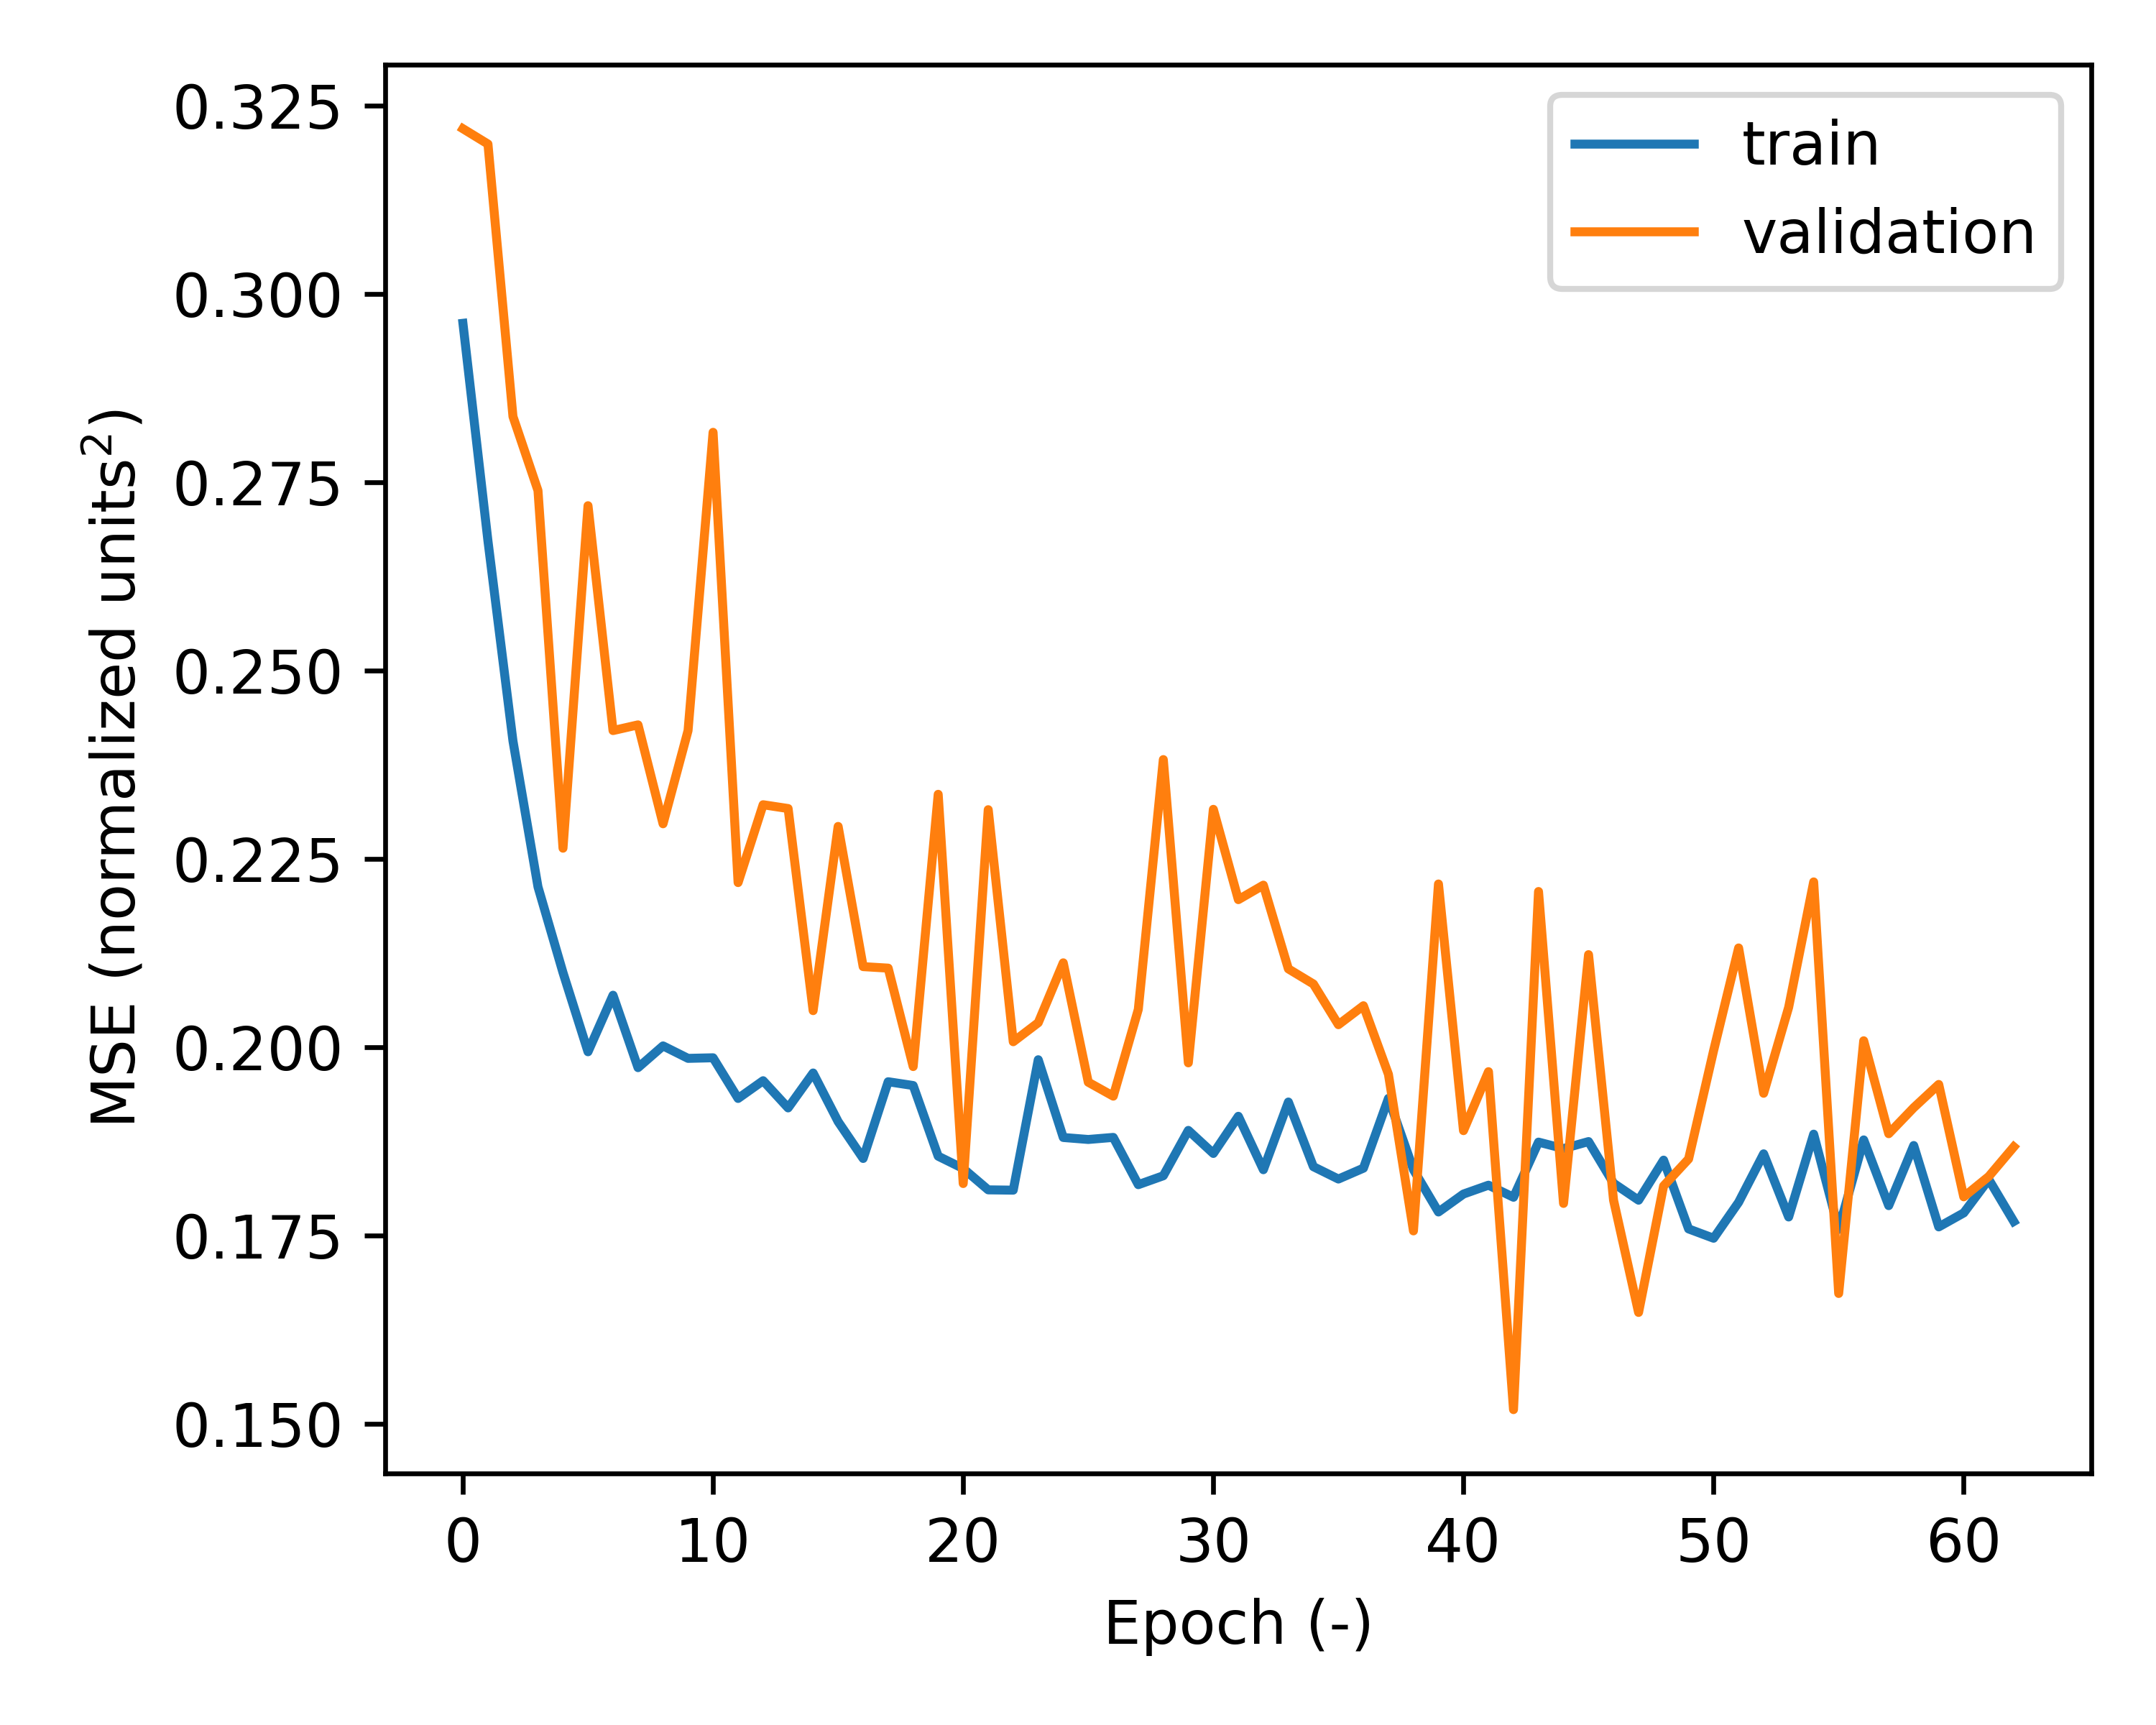
\includegraphics[width=0.88\linewidth,height=5cm]{loss_curve_multi.png}
\caption{Training and validation loss (MSE) of the selected multimodal SNN.}
\label{fig:loss_curve_method}
\end{figure}

\subsection{Hyperparameter Sensitivity}
\rev{The grid results also provide a sensitivity analysis of the LIF parameters and the temporal encoding. Averaging validation loss marginally over the 324 configurations, learning rate had the strongest effect (mean loss 0.826 at $0.0005$ vs. 0.694 at $0.002$). The LIF threshold showed a consistent preference for $\theta=0.8$ over $\theta=1.0$ (0.747 vs. 0.769), while the decay factor had a minor influence (0.754 at $\beta=0.90$ vs. 0.762 at $\beta=0.95$). The temporal parameter $T$ had a weak effect on accuracy (mean loss 0.766, 0.760, and 0.748 for $T=10, 15, 25$), but inference cost grows approximately linearly with $T$, since each additional step implies one more forward pass of spike propagation. Hence $T$ is primarily an energy--latency knob rather than an accuracy knob in this task, and $T=15$ was retained as a balanced operating point.}



\FloatBarrier
